% =============================================================
% Rascunho da seção de Resultados (Hipótese H1) para inclusão no
% artigo final de pgsg_2 (formato elsarticle, periódico-alvo Chemolab).
%
% Este arquivo é um FRAGMENTO -- não compila sozinho como documento
% completo. Deve ser \input{} ou colado dentro do esqueleto elsarticle
% já usado em pgsg_1 (pgsg_v2_paper.tex), na seção \section{Results}.
%
% Dados-fonte: scripts/diagnose_pgsg_gate.py, 4 execuções (16-27/07/2026):
%   - rodada completa: n=6.472 (treino 5.177), p=1.870, max_epochs=200,
%     patience=20 -> best_epoch=0, R2_PLS=0.9044, R2_PGSG=0.9040
%   - diagnóstico n=1.000, seed=42, lr=1e-2, 30 épocas sem early stop
%   - diagnóstico n=1.000, seed=7,  lr=1e-2, 30 épocas sem early stop
%   - diagnóstico n=1.000, seed=42, lr=1e-3, 30 épocas sem early stop
% Figura: h1_diagnostic_val_loss.pdf (gerada por plot_h1_diagnostic.py)
% =============================================================

\subsection{H1: Generalização sem mudança arquitetural}
\label{sec:results-h1}

A Hipótese~1 previa que o \texttt{PGSGModel} de \texttt{pgsg\_1}, aplicado a dados Raman sem qualquer alteração arquitetural, superaria o baseline PLS ($\Delta R^2_{\text{PLS}} > 0$), replicando qualitativamente o resultado obtido em NIR. O resultado observado \textbf{não suporta H1}: na execução completa (\texttt{bioprocess\_substrates}, $n=6.472$, split 80/20, $p=1.870$ bandas, alvo glicose),

\[
\Delta R^2_{\text{PLS}} = R^2_{\text{PGSGv2}} - R^2_{\text{PLS}} = 0{,}9040 - 0{,}9044 = -0{,}0004,
\]

um efeito nulo dentro da precisão numérica do experimento. O treino de $\theta$ parou na \emph{época 0} (\texttt{best\_epoch}~$=0$, com \texttt{patience}~$=20$): nenhuma época subsequente melhorou a \texttt{val\_loss} em relação à inicialização por prior.

\paragraph{Mecanismo diagnosticado.} Uma leitura apressada atribuiria esse resultado ao gradiente vanescente do softmax em alta dimensão, mecanismo já documentado no artigo fundador (\texttt{pgsg\_0}) para $p\approx 281$. Um diagnóstico dedicado (\texttt{scripts/diagnose\_pgsg\_gate.py}), que registra a trajetória completa de \texttt{train\_loss}/\texttt{val\_loss} por época sem interrupção por \emph{early stopping}, mostra um padrão mais específico: \texttt{train\_loss} \emph{decresce} monotonicamente, enquanto \texttt{val\_loss} \emph{cresce} monotonicamente, ambos de forma lenta, a partir da própria época~0 (Figura~\ref{fig:h1-diagnostic}). Isto é, o gradiente não está congelado -- ele se move, mas na direção que ajusta o gate ao ruído do conjunto de treino, não ao sinal generalizável. Com $p=1.870$ graus de liberdade livres em $\theta$, o prior de inicialização já ocupa o ponto de melhor generalização disponível; qualquer passo a partir dele piora o desempenho em validação. Trata-se de \textbf{sobreajuste imediato por sobre-parametrização do gate}, não de gradiente vanescente no sentido estrito (ausência de movimento).

\paragraph{Verificações de robustez.} Para excluir explicações alternativas, o diagnóstico foi repetido com uma segunda semente de particionamento treino/validação (\texttt{seed}~$=7$) e com uma taxa de aprendizado dez vezes menor ($10^{-3}$ em vez de $10^{-2}$), mantendo $p=1.870$ completo e $n=1.000$ amostras (subamostradas apenas em amostras, não em bandas, para preservar a dimensionalidade sob investigação). Em ambos os casos o mesmo padrão qualitativo se repete -- \texttt{val\_loss} monotonicamente crescente desde a época~0 -- descartando tanto a hipótese de um particionamento treino/validação especialmente desfavorável quanto a de um passo de gradiente grande demais como causas do resultado (Figura~\ref{fig:h1-diagnostic}, painel b: a taxa de aprendizado menor apenas desacelera proporcionalmente a mesma trajetória, sem alterar sua direção).

\begin{figure}[htbp]
    \centering
    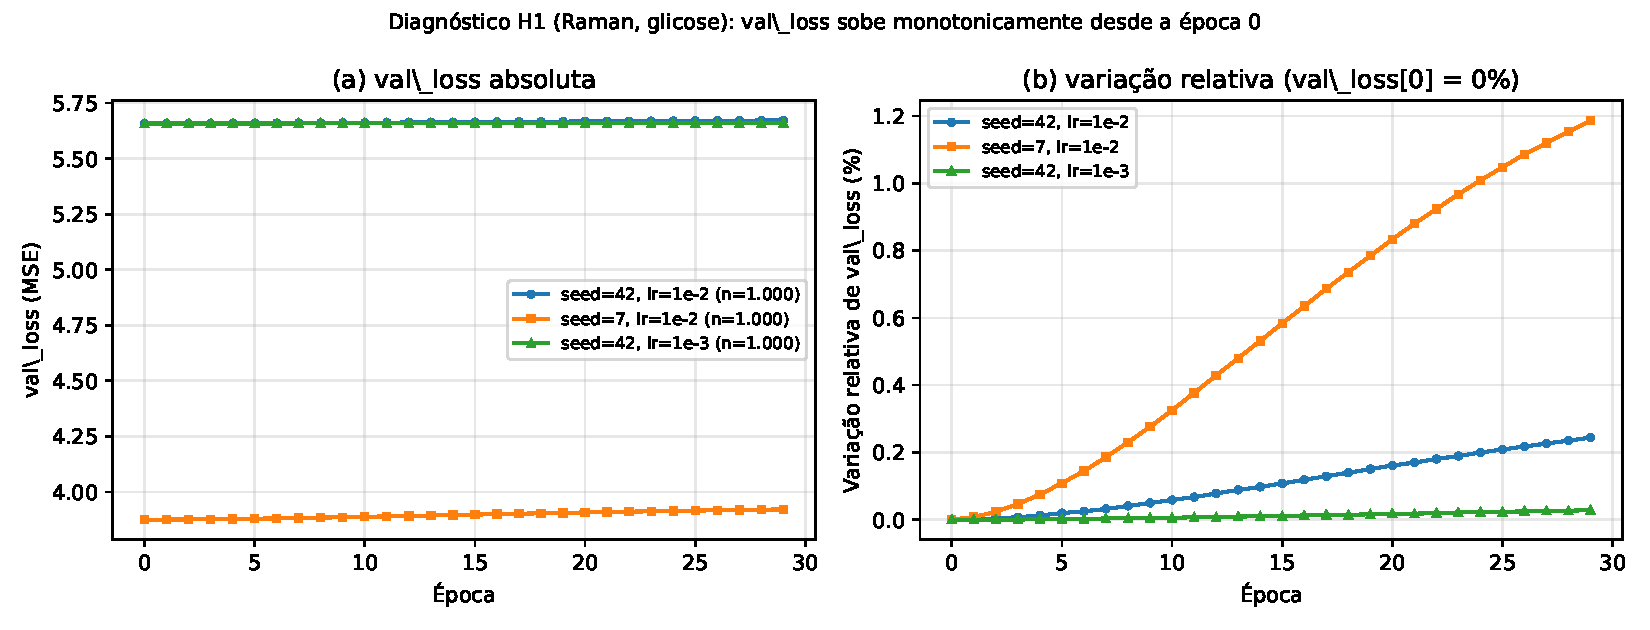
\includegraphics[width=\linewidth]{h1_diagnostic_val_loss.pdf}
    \caption{Trajetória de \texttt{val\_loss} por época em três execuções diagnósticas independentes (bandas Raman completas, $p=1.870$; $n=1.000$ amostras subamostradas apenas em amostras). (a) valores absolutos de \texttt{val\_loss}; (b) variação relativa a partir da época~0, evidenciando que a taxa de aprendizado menor ($10^{-3}$) produz a mesma trajetória de degradação, apenas mais lenta -- não uma trajetória qualitativamente diferente.}
    \label{fig:h1-diagnostic}
\end{figure}

\paragraph{Interpretação.} Este resultado é tratado como um achado científico legítimo, não como uma falha de implementação. Ele expõe uma condição de contorno da arquitetura PGSGv2 não aparente em \texttt{pgsg\_1}: a vantagem do gate aprendido sobre o prior de inicialização parece depender de uma razão amostra/dimensionalidade ($n/p$) mais favorável do que a observada aqui ($n_{\text{treino}}/p \approx 2{,}8$ na rodada completa). Combinado ao teto de desempenho já elevado do PLS não-ponderado ($R^2=0{,}9044$), o espaço para o gate melhorar a predição neste dataset específico é, na prática, inexistente -- o que é consistente com o racional original do programa PGSG, cujo valor esperado é maior em regimes de amostra limitada do que em regimes de amostra abundante como o de \texttt{bioprocess\_substrates}. H1 não é suportada nesta combinação de modalidade e dataset; a Seção~\ref{sec:discussion} discute as implicações para as Hipóteses H2--H5 e para o programa de pesquisa como um todo.
